% !TEX TS-program = pdflatex
% !TEX root = ../LightMicroRep.tex

%************************************************
\chapter{Total Internal Reflection Fluorescence Microscopy}
\label{chp:TIRF}
%************************************************
\numberwithin{figure}{section}
%----------------------------------------------------------------------------------------
%	INTRODUCTION
%----------------------------------------------------------------------------------------

\section{Introduction}

\paragraph{Aim} To observe adhesion between cells and the contact between cell-surface.
\\

Total Internal Reflection Fluorescence Microscopy (TIRF) allows imaging of fluorescent molecules located close to the glass/water (or glass/specimen) interface. 
Depending on the excitation wavelength and objective NA, the thickness of the excitation depth, which is called the evanescent field, can be less than 100 nm from the solid surface. 
In comparison, the thickness of a confocal image section is approximately 500 nm \cite{Fish2009}. 
However the disadvantage is that the section is confined to a single-plane immediately adjacent to the glass \cite{Sanderson2014}.

In TIRF, excitation light is beamed thorugh a glass substrate in direction of an aqueous specimen at a certain angle called the critical angle, at which total internal reflection occurs. 
This is due to the difference of recfractive index between glass and water. This produces an evanescent wave (an electromagnetic field) in the aqueous phase. 
The evanescent field penetration depends on light wavelength, difference of refractive index, and the angle of incidence. 
Since the penetration of the evanescent field rapidly decays, only the fluorophores near the glass-liquid interface are excited, allowing a form of optical sectioning. 

To reach an angle of incidence that is greater than the critical angle, TIRF microscopy requires a high NA (> 1.45). This can be achieved by using immersion oil.

%----------------------------------------------------------------------------------------
%	METHODS
%----------------------------------------------------------------------------------------

\section{Methods}

The specimen in this experiment is \textit{Dictyostelium discoideum}, an amoeba, treated with the fluorescent marker Lim-GFP (Green Fluorescent Protein). 
This fluorescent marker is excited by blue laser (490 nm) and emits at 510 nm. 

The measurement was conducted using the inverted microscope Olympus IX71. 
A semiconductor laser was used to excite the fluorescent marker during imaging.
%----------------------------------------------------------------------------------------
%	RESULTS AND DISCUSSION
%----------------------------------------------------------------------------------------
\section{Results and Discussion}
Lim-GFP is bound to the actin network of the cell due to the lim domain. Other parts of the cell can be marked using Lim-RFP.
The size of this amoeba cell is normally 10-20 $\mu$m.

\begin{figure}[h]
\centering
\subfloat[Normal\label{anorm}]{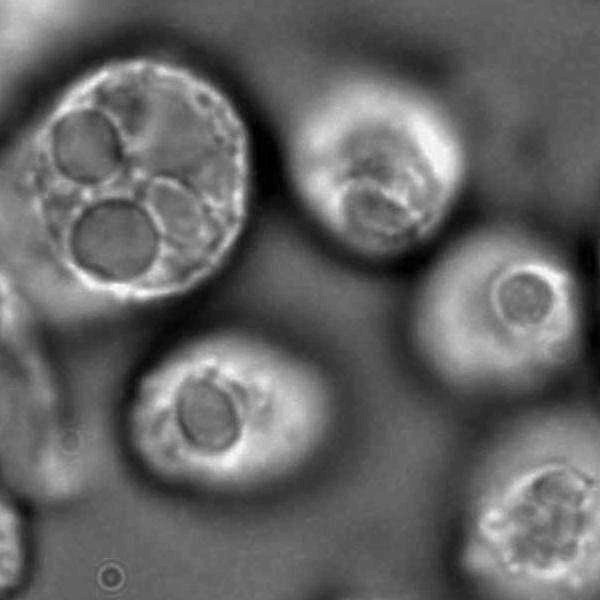
\includegraphics[width=.45\columnwidth]{Exp_4_TIRF/Figures/c2_cropped_grey8_norm0}} \hspace{0.1mm}
\subfloat[TIRF\label{atirf}]{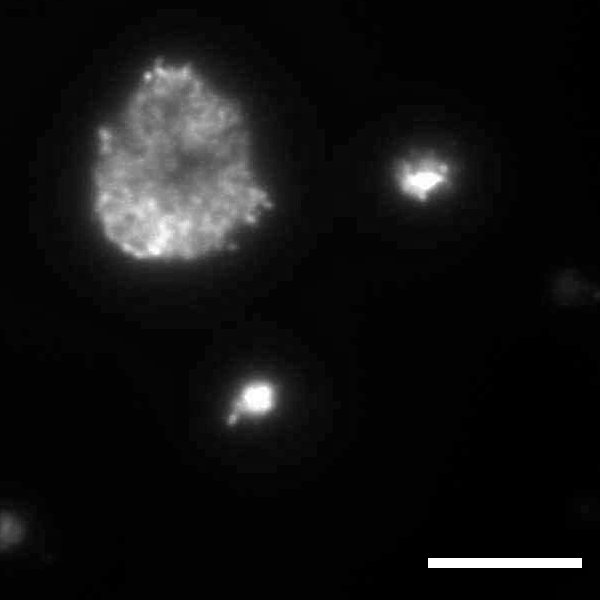
\includegraphics[width=.45\columnwidth]{Exp_4_TIRF/Figures/c1_cropped_grey32incon_scale10um}} \\
\caption[a: normal, b: opsec.]{Side-by-side comparison of the same area of \textit{Dictyostelium discoideum} imaged with normal and TIRF mode. 
Objective lens: UAPON 100$\times$ 1.49 oil immersion. 
Scalebar is 10 $\mu$m.} 
\label{fig:amoebatirf}
\end{figure}

From a direct comparison between the images (Fig.~\ref{fig:amoebatirf}) it can be seen that through normal mode, there are many that cells can be observed, however the TIRF mode only presents the cells, or a part (section) of the cells, that are \textit{attached} to the slide, avoiding fluorescence excitation from other parts of the cell. 
Due to this, the images produced by this method have good signal-to-noise ratio with minimal fluorescence from out-of-focus planes. 
This is demonstrated by the vacuoles that can normally be seen in Fig.~\ref{anorm}. These vacuoles which are located usually around the center of cells are not observable anymore in TIRF mode (Fig.~\ref{atirf}).

The cells in the specimen were newly cultivated, which may account for the seemingly smaller size of the cells in the image. 
This may also play a part in the fact that the cells can move more freely and not very much attached to the slide. 
Since the cells were alive, the displacement of the cells can be observed during the imaging process when the experimenter changed the mode of imaging from normal to TIRF mode and adjusted the angle of reflection.

Comparing Fig.~\ref{atirf} and Fig.~\ref{fig:amoebatirfb}, the varying size of the cells are evident. 
On some of the cells, there are protruding parts that can be seen, these could be the pseudopods of the amoeba cells.

\begin{figure}[h]
\centering
\subfloat{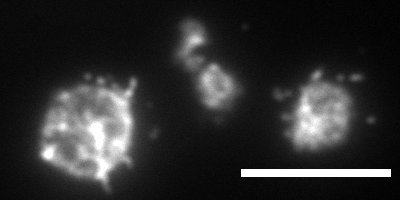
\includegraphics[width=.6\columnwidth]{Exp_4_TIRF/Figures/b1_incon_scale10um}}
\caption{Another part of the same specimen. 
Objective lens: UAPON 100$\times$ 1.49 oil immersion. 
Scalebar is 10 $\mu$m.}
\label{fig:amoebatirfb}
\end{figure}
 

%----------------------------------------------------------------------------------------
%	BIBLIOGRAPHY
%----------------------------------------------------------------------------------------

%\renewcommand{\refname}{\spacedlowsmallcaps{References}} % For modifying the bibliography heading

%\bibliographystyle{unsrt}

%\bibliography{Biblio} % The file containing the bibliography

%\printbibliography[heading=subbibintoc]
%\end{refsection}
